\section{双线性型与线性映射}

设 \((\mathrm{F}_{1},\mathrm{G}_{1}),(\mathrm{F}_{2},\mathrm{G}_{2})\) 是两对处于分离对偶中的（实或复）向量空间（TVS, II, §6, No.~1）；假定这些空间中的每一个都装备相应的弱拓扑（出处同上， No.~2）；若 A 与 B 是这些空间中的任意两个，我们照例用 \(\mathcal{L}(\mathrm{A};\mathrm{B})\) 表示 A 到 B 中的连续线性映射所成的向量空间，用 \(\mathfrak{B}(\mathrm{A},\mathrm{B})\) 表示 \(\mathrm{A}\times \mathrm{B}\) 上分别连续的双线性型所成的向量空间。

设 \(\Phi\) 是 \(\mathrm{F}_1\times \mathrm{F}_2\) 上任意一个分别连续的双线性型，则 \(x_{1}\mapsto \Phi (x_{1},x_{2})\) 是 \(\mathrm{F}_1\) 上的连续线性形式，因此存在唯一的一个元素 \(^r\Phi (x_2)\in \mathbf{G}_1\) ，使得

\[
\Phi (x _ {1}, x _ {2}) = \langle x _ {1}, ^ {r} \Phi (x _ {2}) \rangle\tag{1}
\]

对 \(x_{1} \in F_{1}\) 、 \(x_{2} \in F_{2}\) 成立（TVS, III, §5, No.~1, (1)）。此外，这个公式表明映射 \(x_{2} \mapsto {}^{r}\Phi(x_{2})\) 对 \(F_{2}\) 与 \(G_{1}\) 的（弱）拓扑是线性且连续的。反之，对 \(F_{2}\) 到 \(G_{1}\) 中的每个连续线性映射 u ， \((x_{1}, x_{2}) \mapsto \Phi(x_{1}, x_{2}) = \langle x_{1}, u(x_{2}) \rangle\) 是 \(F_{1} \times F_{2}\) 上的一个分别连续的双线性型，且 \(^{r}\Phi = u\) 。这样便定义了一个同构 \(r : \Phi \mapsto {}^{r}\Phi\) （ \(\mathfrak{B}(F_{1}, F_{2})\) 到 \(\mathcal{L}(F_{2}; G_{1})\) 上的同构），称为典范同构。

类似地，公式

\[
\Phi (x _ {1}, x _ {2}) = \langle^ {l} \Phi (x _ {1}), x _ {2} \rangle\tag{2}
\]

定义了一个典范同构 \(l: \Phi \mapsto {}^{l} \Phi\) （ \(\mathfrak{B}(F_{1}, F_{2})\) 到 \(\mathcal{L}(F_{1}; G_{2})\) 上的同构）；并且显然有交换图

\pandocbounded{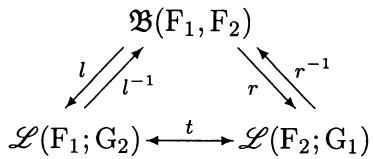
\includegraphics[keepaspectratio]{images/part003_fb3d81cd.jpg}}

其中 t 是转置同构 \(u \mapsto {}^{t}u\) 。鉴于 \(G_{1}\) 与 \(G_{2}\) 上弱拓扑的定义，还可直接看出：当 \(\mathfrak{B}(F_{1}, F_{2})\) 、 \(\mathcal{L}(F_{1}; G_{2})\) 与 \(\mathcal{L}(F_{2}; G_{1})\) 装备逐点收敛拓扑时，前一图中的同构是拓扑向量空间结构之间的同构。

现在设 E 、 F 是两个 Hausdorff 局部凸空间， \(E'\) 、 \(F'\) 是它们的对偶；我们用 \(E_{\sigma}\) 、 \(F_{\sigma}\) 表示装备弱化拓扑 \(\sigma(\mathrm{E}, \mathrm{E}')\) 、 \(\sigma(\mathrm{F}, \mathrm{F}')\) 的空间 E 、 F ，用 \(E_{s}'\) 、 \(F_{s}'\) 表示空间 \(E'\) 、 \(F'\) （装备弱拓扑 \(\sigma(\mathrm{E}', \mathrm{E})\) 、 \(\sigma(\mathrm{F}', \mathrm{F})\) ）。于是，前面的注记在三个空间 \(\mathfrak{B}(\mathrm{E}_{\sigma}, \mathrm{F}_{s}')\) 、 \(\mathcal{L}(\mathrm{E}_{\sigma}; \mathrm{F}_{\sigma})\) 与 \(\mathcal{L}(\mathrm{F}_{s}'; \mathrm{E}_{s}')\) 之间建立了典范同构，也在三个空间 \(\mathfrak{B}(\mathrm{E}_{\sigma}, \mathrm{F}_{\sigma})\) 、 \(\mathcal{L}(\mathrm{E}_{\sigma}; \mathrm{F}_{s}')\) 与 \(\mathcal{L}(\mathrm{F}_{\sigma}; \mathrm{E}_{s}')\) 之间建立了典范同构。我们将注意到， \(\mathfrak{B}(\mathrm{E}_{\sigma}, \mathrm{F}_{\sigma})\) 也等于空间 \(\mathfrak{B}(\mathrm{E}, \mathrm{F})\) ，即 \(E \times F\) 上分别连续双线性型所成的空间（ E 与 F 装备其原来的拓扑），因为 E （相应地， F ）上的每个连续线性形式在 \(E_{\sigma}\) （相应地， \(F_{\sigma}\) ）上连续，反之亦然（TVS, II, §6, No.~1 与 No.~2, 命题 3）。

设 \(\mathcal{B}(\mathrm{E},\mathrm{F})\) 是 \(\mathbf{E}\times \mathbf{F}\) 上连续双线性型所成的空间（ E 与 F 装备其原来的拓扑）；则 \(\mathcal{B}(\mathrm{E},\mathrm{F})\subset \mathfrak{B}(\mathrm{E},\mathrm{F})\) 。

命题 1. --- 双线性型 \(\Phi \in \mathfrak{B}(\mathrm{E},\mathrm{F})\) 属于 \(\mathcal{B}(\mathrm{E},\mathrm{F})\) 的充要条件是：存在 E 的一个 0 的邻域，它在 \(^l\Phi\) 下的像是 \(\mathbf{F}'\) 的一个等度连续子集。

因为，说 \(\Phi\) 连续，意思是存在 E （相应地， F ）中 0 的一个均衡凸邻域 V （相应地， W ），使得 \(|\Phi(x,y)| \leqslant 1\) （对 \(x \in V\) 、 \(y \in W\) ）；这可写成 \(|\langle^{l}\Phi(x), y \rangle| \leqslant 1\) （对 \(x \in V\) 、 \(y \in W\) ），或者写成 \(^{l}\Phi(V) \subset W^{\circ}\) ；由此即得命题，因为考虑到 \(F'\) 的每个等度连续子集都含于 F 中 0 的某个邻域的极集。

推论. --- 若 \(\Phi\) 是 \(\mathbf{E} \times \mathbf{F}\) 上的连续双线性型，则 \(^l\Phi\) 是 \(\mathbf{E}\) 到强对偶 \(\mathbf{F}_b'\) （ \(\mathbf{F}\) 的强对偶）中的连续线性映射。此外，若 \(\mathbf{E}\) 与 \(\mathbf{F}\) 是赋范空间，则 \(\|^l\Phi\| = \| \Phi \|\) 。

第一个断言由命题 1 以及 \(F_{b}^{\prime}\) 中 0 的每个邻域都吸收 \(F^{\prime}\) 的每个等度连续子集这一事实得出。若 E 与 F 赋范，则

\[
\begin{array}{c} \| \Phi \| = \sup _ {\| x \| \leqslant 1, \| y \| \leqslant 1} | \Phi (x, y) | = \sup _ {\| x \| \leqslant 1} \Big (\sup _ {\| y \| \leqslant 1} \big | \langle^ {l} \Phi (x), y \rangle \big | \Big) \\ = \sup _ {\| x \| \leqslant 1} \| ^ {l} \Phi (x) \| = \| ^ {l} \Phi \|, \end{array}
\]

由此得第二个断言。

交换 E 与 F 的角色，对线性映射 \(r\Phi\) 可得到与命题 1 及其推论类似的结果；我们把这些结果的叙述留给读者。

